Ferner bietet Maven die Möglichkeit, eigene Plugins zu erstellen, womit Aufgaben und Arbeitsabläufe einfach in den Projektablauf integriert werden können, die spezifisch für das jewelige Unternehmen benötigt werden. \cite[S. 3]{varanasi_introducing_2019}

Basierend auf dem Rahmen dieser Arbeit, OSS in den DevOps-Softwareentwicklungsprozesses zu integrieren, wurde diese Möglichkeit für den PoC aufgegriffen. 

Demgemäß wurde eine entsprechende OSS als ein Maven Plugin \cite{allberg_ayoyabayoy-maven-license-verifier-plugin_2021} innerhalb des PoCs auf GitHub, einer der bekanntesten Plattformen für Quellcode-Datenbanken und deren Versionverwaltung, heruntergeladen und für den entsprechenden Verwendungszweck angepasst.

\subsubsection{Workflow Maven}

Um ein besseres Verständnis zu ermöglichen, wird zunächst auf die generelle Funktionsweise von Maven näher eingegangen. 

\begin{figure}[h]
    \centering
    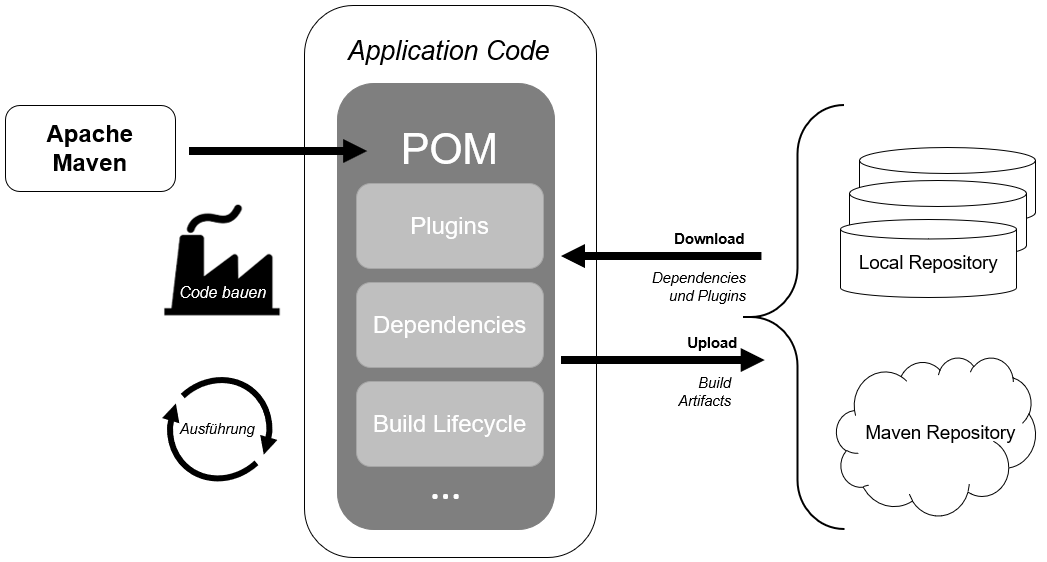
\includegraphics[scale=0.6]{Bilder/Workflow_Maven.png}
    \caption{Funktionsweise von Maven, angelegt an \cite{guntur_understanding_2020}}
\end{figure}

%Repository/POM
Um Projektbeziehungen und Abhängigkeiten (engl: Dependencies) zu konfigurieren, baut die Funktionsweise von Maven grundsätzlich auf dem 'Project Object Model' (kurz: POM), um das Projekt zu verwalten.

Die POM wird innerhalb der Datei pom.xml gespeichert, die wiederrum im Projektverzeichnis liegt. 

Die POMs erben alle definierten Eigenschaften von der Super-POM, welches die Standardkonfigurationen, Plugins und Verzeichnisse enthält. 

Ferner verwendet Maven das 'Local Repository'. 

In diesem lokalen Verzeichnis werden alle Bibliotheken abgelegt, die für die Erstellung des Builds benötigt werden. 

Sollten neue Bibliotheken oder neue Versionen der vorhandenen Bibliotheken hinzugefügt werden, wird das Repository anhand dessen aktualisiert oder die betreffenden Bibliotheken kopiert. 

Zur Zerlegung der Abhängigkeiten überprüft Maven, ob sich die benötigten Daten bereits innerhalb des Local Repositorys befinden. 

Ist dies der Fall, wird die Datei, ohne die Erstellung einer Kopie im Verzeichnis, innerhalb des Repositorys verwendet.

% Kann keine lokale Zerlegung der Abhängigkeit erfolgen, versucht Maven, 



% Kann die Abhängigkeit nicht lokal aufgelöst werden, versucht Maven, sich mit einem konfigurierten Maven-Repository im Intranet oder Internet zu verbinden und von dort die Dateien in das lokale Repository zu kopieren, um sie von nun an lokal verwenden zu können.

% Firmenweite über das Intranet ansprechbare Maven-Repositorys dienen dazu, selbst entwickelte oder gekaufte Bibliotheken und Frameworks firmenweit allen Projekten zur Verfügung zu stellen. 

%Verzeichnis


%Funktionsweise
% Prinzipiell geht Maven von wiederholenden Aufgaben anhand festgelegter Lifecycles aus. 

% Der Standard-Lifecycle ist der Build-Lifecycle, der die feste Reihenfolge enthält, die zur  Erstellung  eines  Builds nötig  ist. Da  die  Reihenfolge  der  Phasen  von  Maven feststeht,  ist  außerdem  keine  Analyse bzw.  Erstellung von  Build-Skripten  nötig.

% Die Maven-Befehle führen Teile des Projektobjektsmodells aus. 

\paragraph{Build-Lifecycle}

\paragraph{Abhängigkeiten verwalten mittels Dependencies-Dateien}

\paragraph{Plugins in Maven}

\subsubsection{Entwurf PoC basierend auf einem Maven-Plugin}
%Idee: Lizenzen als eine Datei zu beschreiben und mit den Lizenzen die sich in den Dependency-Dateien befinden, zu vergleichen 



